\documentclass[compress, smaller, serif, 9pt]{beamer}


\mode<presentation>
{
  \usetheme{Montpellier}
  %\setbeamercovered{transparent}
  % or whatever (possibly just delete it)
}
% or whatever
%\setbeamertemplate{footline}[frame number]
\beamertemplatenavigationsymbolsempty
\beamertemplatetransparentcovereddynamic

\usepackage[english,frenchb]{babel}
\usepackage[utf8]{inputenc}
% or whatever
%\setbeamertemplate{footline}[frame number]
\beamertemplatenavigationsymbolsempty
\beamertemplatetransparentcovereddynamic
\usefoottemplate{%
       \tinycolouredline{blue!03}%
       {
           \hspace{11.5cm}{\color{black!50} {\insertframenumber $/$ \inserttotalframenumber} \hfill}
       }%
}


% Definitions
%\input{def}
% Raccourcis
%\input{raccourci}

% Beamer settings
%\setbeamercolor{structure}{fg=myem!120}
%\setbeamercolor{example}{bg=LightYell,fg=StroYell}

% \setbeamercolor{alerted text}{fg=lightred}
% \setbeamertemplate{blocks}[rounded][shadow=true]
% \newcommand{\exampletext}[1]{{\usebeamercolor[fg]{example text} #1}}
% \newcommand{\structuretext}[1]{{\usebeamercolor[fg]{structure} #1}}
% \usefonttheme[onlymath]{serif}
% \renewcommand{\thefootnote}{\fnsymbol{footnote}}

%\setbeamerfont{sidebar}{5pt}

\usepackage{amssymb}
%\usepackage[T1]{fontenc}
\usepackage{amsmath,amsthm,bm}
\usepackage{pgf}


\graphicspath{{./Figs/S04/},{./Figs/S03/}}

\usepackage[normal]{subfigure}
\newcommand{\goodgap}{%
    \hspace{\subfigtopskip}%
    \hspace{\subfigbottomskip}}

% les macros
\newcommand{\exampletext}[1]{{\usebeamercolor[fg]{example text} #1}}
\newcommand{\structuretext}[1]{{\usebeamercolor[fg]{structure} #1}}

\newcommand{\bydef}{\stackrel{{def}}{=}}
\newcommand{\ici}{\tcb{$\blacktriangleright \;$}}
\newcommand{\icir}{\alert{$\blacktriangleright \;$}}
\newcommand{\iciex}{\exampletext{$\blacktriangleright \;$}}
\usepackage{pifont}
\newcommand{\doigt}{\structuretext{\noindent \Pisymbol{pzd}{43}}}
\newcommand{\doigtr}{\alert{\noindent \Pisymbol{pzd}{43}}}
\newcommand{\doigtex}{{\exampletext{\noindent \Pisymbol{pzd}{43}}}}


\newcommand{\bx}{{\boldsymbol{x}}}
\newcommand{\bbeta}{{\boldsymbol{\beta}}}
\newcommand{\balpha}{{\boldsymbol{\alpha}}}
\newcommand{\bxi}{{\boldsymbol{\xi}}}


\DeclareMathOperator{\var}{var}
\DeclareMathOperator{\cov}{cov}
\DeclareMathOperator{\trace}{trace}
\DeclareMathOperator{\rank}{rank}
\DeclareMathOperator{\logit}{logit}
\DeclareMathOperator{\sign}{sign}


\setbeamerfont{block title}{size={\normalsize}}


\title[Statistical Learning]{Machine/Statistical Learning}

\subtitle{Lecture 4: Prototype/black-box approaches\\
SVM: Support Vector Machine}


%\author[Florent Chatelain]{Florent Chatelain}
\institute{Filière SICOM, 3A}
%\logo{\includegraphics[width=.2\textwidth]{logoE3}}

\date{}



%

\begin{document}

\maketitle

\begin{frame}{Support Vector Machine (SVM)}

Theory elaborated in the early 1990's (Vapnik {\em et al}) based on the idea of {\structuretext{ 'maximum margin'}}

\begin{itemize}
 \item deterministic criterion learned on the training set $\leftarrow$  \structuretext{supervised classification}
 \item[\doigt] general, i.e. \structuretext{model free}, linear classification rule
 \item[\doigt] classification rule is linear in a transformed space of higher (possible infinite) dimension than the original input feature/predictor space
\end{itemize}

 
\end{frame}


\begin{frame}{Linear discrimination and Separating hyperplane}

  \begin{block}{Binary classification problem}
  \begin{itemize}
     \item $X \in \mathbb{R}^p$
     \item $Y \in \{-1,1\} \leftarrow $ 2 classes
     \item Training set $(x_i,y_i)$, for $i=1,\ldots,n$
  \end{itemize}
  \end{block}

 Defining a \structuretext{linear} discriminant function $h(x)$ 
 $\Leftrightarrow$ defining a separating \structuretext{hyperplane} $\mathcal{H}$ with equation\\
  \begin{minipage}{.4\textwidth}
\begin{center}
                   $$
 \boldsymbol{x}^T \boldsymbol{\beta} + \beta_0 = 0, 
 $$
\end{center}
\end{minipage}
\quad
 \begin{minipage}{.3\textwidth}
  \begin{center}
   \includegraphics[width=\textwidth]{geom_hyperplane_wopoint.pdf}
  \end{center}
 \end{minipage}


\begin{itemize}
 \item $\boldsymbol{\beta} \in \mathbb{R}^p$ is the normal vector (vector normal to the hyperplane $\mathcal{H}$),
 \item $\beta_0 \in \mathbb{R}$ is the intercept/offset (regression or geometrical interpretation)
 \item[\doigt] $\mathcal{H}$ is an {\em affine set} of codimension $1$
 \item[\doigt] $h(x)\equiv \boldsymbol{x}^T \boldsymbol{\beta} + \beta_0$ is the associated (linear) discriminant function
\end{itemize}

 
\end{frame}





\begin{frame}{Separating hyperplane and prediction rule}

 For a given separating {hyperplane} $\mathcal{H}$ with equation \medskip \\
  \begin{minipage}{.4\textwidth}
\begin{center}
                   $$
 \boldsymbol{x}^T \boldsymbol{\beta} + \beta_0 = 0, 
 $$
\end{center}
\end{minipage}
\quad
 \begin{minipage}{.3\textwidth}
  \begin{center}
   \includegraphics[width=\textwidth]{geom_hyperplane_wopoint.pdf}
  \end{center}
 \end{minipage} \bigskip \\
 the \structuretext{prediction rule} can be expressed as
\begin{itemize}
 \item $\widehat{y}=+1$, if $h(\boldsymbol{x})= \boldsymbol{x}^T \boldsymbol{\beta} + \beta_0 \ge 0$,
 \item  $\widehat{y}=-1$, otherwise,
\end{itemize}
or in an equivalent way:
\begin{align*}
 \widehat{y} &\equiv G(\boldsymbol{x}) = \structuretext{ \sign{\left[  \boldsymbol{x}^T \boldsymbol{\beta} + \beta_0 \right]} }
\end{align*}

\begin{itemize}
 \item[Rk:] $\boldsymbol{x}$ if correctly classified when $G(\boldsymbol{x})=y$ $\Leftrightarrow$ 
 $y \left(  \boldsymbol{x}^T \boldsymbol{\beta} + \beta_0 \right )  \ge 0$
 \end{itemize}

\end{frame}



\section{Separable case}

\begin{frame}
  \frametitle{Separating Hyperplane: separable case}
  
  %\begin{block}{Binary supervised classification}
%   $X \in \mathbb{R}^p$, $Y \in \{-1,1\}$, Training set $(x_1,y_1),\ldots,(x_n,y_n)$
  %\end{block}

  \medskip
  
  \structuretext{Linear separability assumption:} 
  $\exists \boldsymbol{\beta}  \in \mathbb{R}^p$ and $\beta_0 \in \mathbb{R}$ s.t. the hyperplane 
  $\boldsymbol{x}^T \boldsymbol{\beta} + \beta_0 = 0$ 
  perfectly separates 
  the two classes on the training set:
  $$\begin{displaystyle}       y_k  \left(  x^T_k \boldsymbol{\beta} + \beta_0 \right) \ge 0, \quad \textrm{ for } k=1,\ldots,n,
  \end{displaystyle}$$

%  \vspace{-2mm}
\begin{block}{Separable case ($p=2$ example)}
\begin{minipage}{.6\textwidth}
  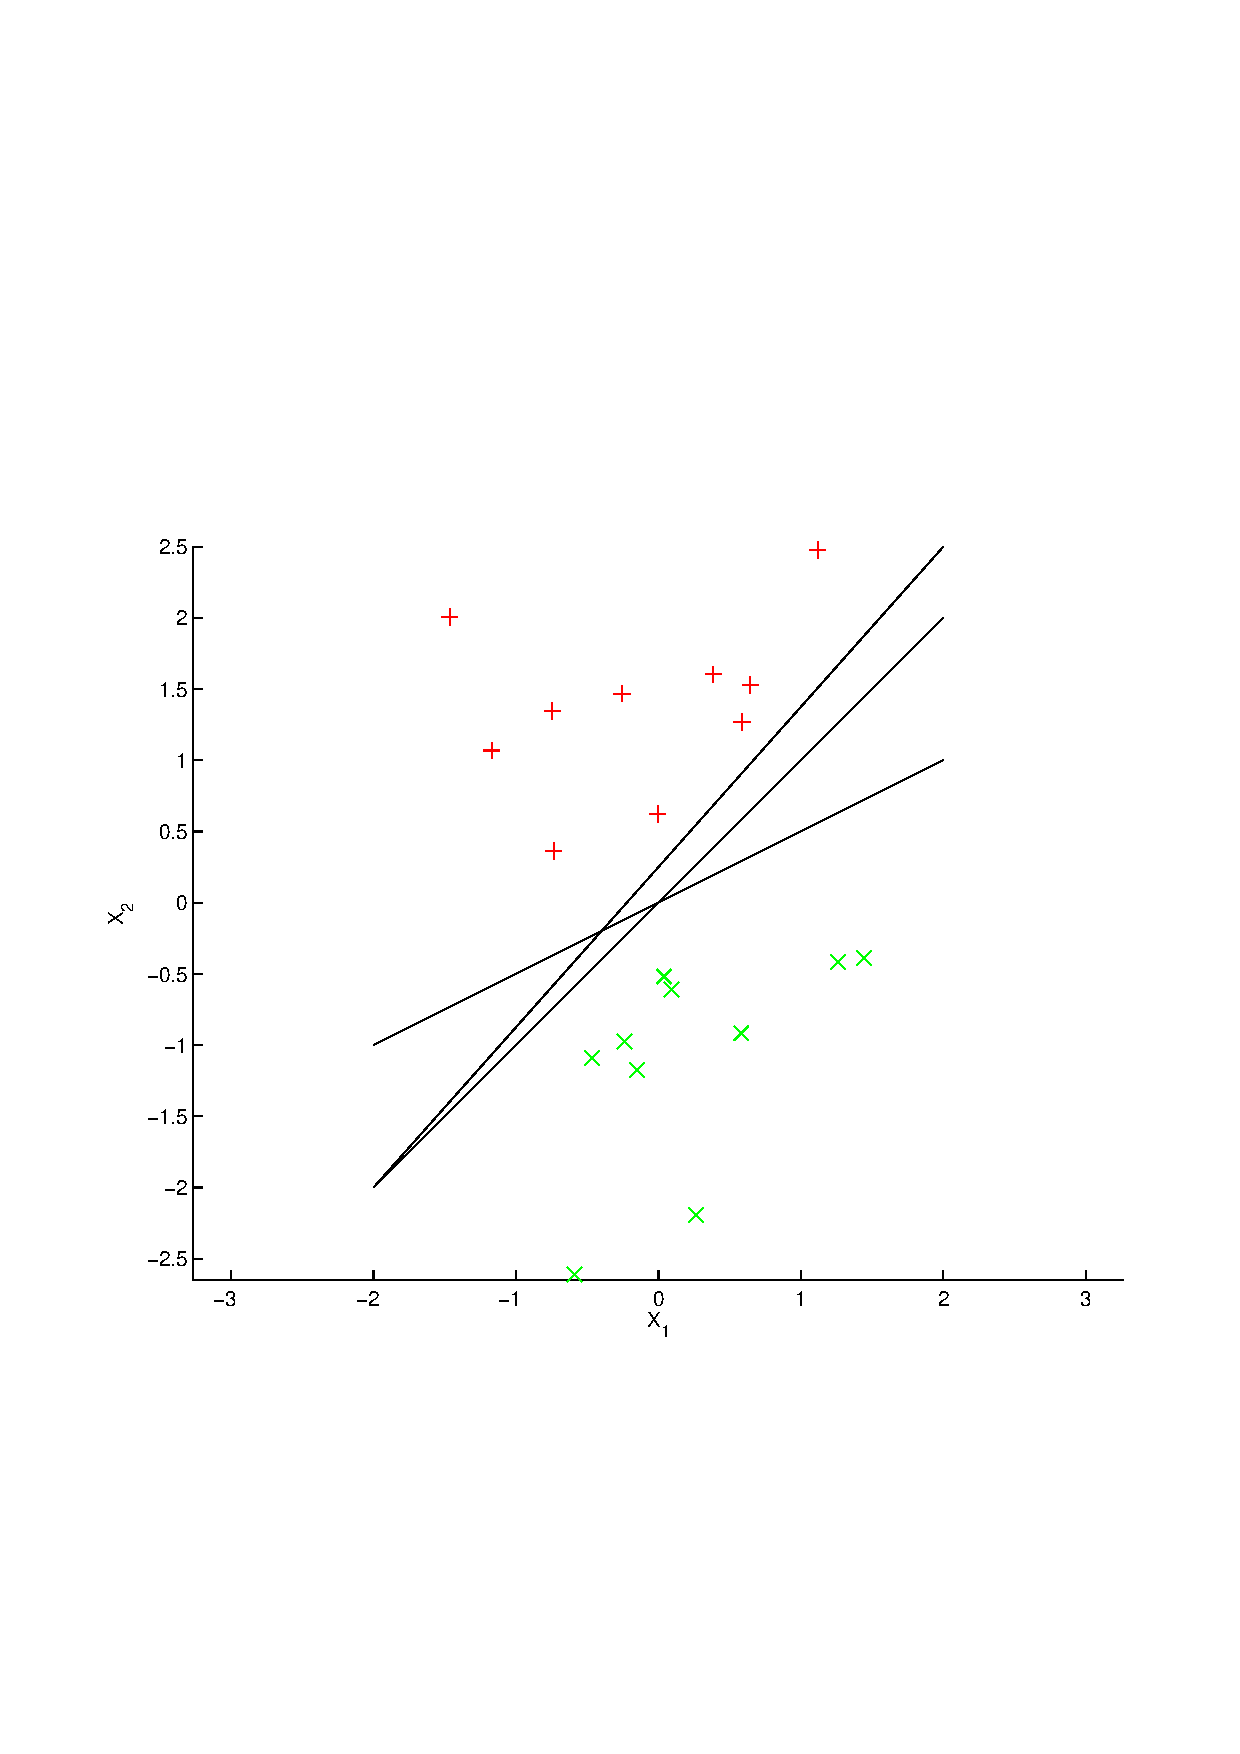
\includegraphics[width=.87\textwidth]{hyperplans_separateur.pdf}
\end{minipage}
\begin{minipage}{.39\textwidth}
  \begin{itemize}
     \item[\alert{Pb:}] infinitely \alert{many} possible perfect \alert{separating hyperplanes} $\boldsymbol{x}^T\boldsymbol{\beta} + \beta_0=0$
     \item[\doigt] Find the 'optimal' separating hyperplane
  \end{itemize}
  \end{minipage}
\end{block}

\end{frame}

\begin{frame}
   \frametitle{Maximum margin separating hyperplane (separable case)}
   
   
   Distance of a point $\boldsymbol{x_k}$ to an hyperplane  $\mathcal{H}$ s.t. $\boldsymbol{x}^T \boldsymbol{\beta} + \beta_0 = 0$, 
   $$d(x_k,\mathcal{H}) \equiv \min_{\boldsymbol{x}} \left\{ \| \boldsymbol{x} - \boldsymbol{x}_k \| \ : \ 
    \boldsymbol{x}^T \boldsymbol{\beta} + \beta_0 = 0 \right\}$$

   
   \begin{block}{Maximum margin principle}
   We are interested in the 'optimal' perfect separating hyperplane maximizing the distance $M>0$, called the \structuretext{margin},
   between the samples of each class and the separating hyperplane
   \begin{itemize}
      \item[$\Rightarrow$] Find  $\boldsymbol{\beta}  \in \mathbb{R}^p$ and $\beta_0 \in \mathbb{R}$ s.t. the margin
    $$
      \structuretext{M}= \min_{1\le k \le n} \left\{ d(x_k,\mathcal{H}) \right\}
    $$
    \end{itemize}
    is \structuretext{maximized}
      \end{block}
  \end{frame}    
  
  
  \begin{frame}
   \frametitle{Signed distance}
   \medskip
   
  \begin{minipage}{.65\textwidth}
  From the orthogonality principle, 
  $$d(x_0,\mathcal{H})=\left\|  \boldsymbol{x}_0 - \widehat{\boldsymbol{x}}_0 \right\|,$$
  where $\widehat{\boldsymbol{x}}_0$ is the orthogonal projection of $\boldsymbol{x}_0$ on $\mathcal{H}$
\end{minipage}
\hfill
 \begin{minipage}{.3\textwidth}
  \begin{center}
   \includegraphics[width=\textwidth]{geom_hyperplane.pdf}\\
    $\widehat{\bx}_0 \in \mathcal{H} \Rightarrow - \widehat{\bx}_0^T\bbeta=\beta_0$
  \end{center}
 \end{minipage} \bigskip \\
 \begin{itemize}
  \item[$\Rightarrow$] $\boldsymbol{x}_0 - \widehat{\boldsymbol{x}}_0$ and  $\boldsymbol{\beta}$ are collinear,
   \item[$\Rightarrow$] $\boldsymbol{x}_0 - \widehat{\boldsymbol{x}}_0= \underbrace{\langle \bx_0 - \widehat{\bx}_0, \bbeta^{*} \rangle}_{\textrm{signed distance}} \bbeta^{*}$, where $ \bbeta^{*}= \frac{\bbeta}{\|\bbeta\|}$, %and $\widehat{\bx}_0^T\boldsymbol{\beta} + \beta_0=0$ since $\widehat{\bx}_0 \in \mathcal{H}$
    \item[$\Rightarrow$] $\begin{displaystyle}
    \textrm{\structuretext{signed distance} }= \left( \bx_0 - \widehat{\bx}_0\right)^T \frac{\bbeta}{\|\bbeta\|}= 
    \frac{\bx_0^T \bbeta - \widehat{\bx}_0^T \bbeta}{\|\bbeta\|}= \structuretext{\frac{\bx_0^T \bbeta +\beta_0}{\|\bbeta\|}},\end{displaystyle}$ 
 \end{itemize}
\begin{block}{Remarks}
  \begin{itemize}
 %\item the last equality comes from $\widehat{\bx}_0 \in \mathcal{H}$
    \item %$\langle \bx_0 - \widehat{\bx}_0, \bbeta^{*} \rangle\ge 0$ iff $\bx_0 - \widehat{\bx}_0$ and $\bbeta$ have same orientations, and  
    $|\langle \bx_0 - \widehat{\bx}_0, \bbeta^{*} \rangle|= \| \bx_0 - \widehat{\bx}_0 \|= d(\bx_0,\mathcal{H}) \leftarrow$  ``signed distance''
    \item for any perfect separating hyperplane $y_k \langle \bx_k - \widehat{\bx}_k, \bbeta^{*} \rangle= \frac{1}{\|\bbeta\|} y_k ( \bx_k^T \bbeta +\beta_0)  \ge 0$, for $k=1,\ldots,n$, 
 \end{itemize}
     \end{block}
  \end{frame}    
  
  
    \begin{frame}
   \frametitle{Canonical separating hyperplane}

   For any perfect separating hyperplane, for  $k=1,\ldots,n$
   $$y_k \langle \bx_k - \widehat{\bx}_k, \bbeta^{*} \rangle= d(x_k,\mathcal{H})$$ 
   Hence, the 
   margin reads
   $$
   M \equiv \min_{1\le k\le n} \left\{  d(x_k,\mathcal{H}) \right\} =  \frac{1}{\| \bbeta \| } \min_{1\le k\le n} \left\{ y_k ( \bx_k^T \bbeta +\beta_0)  \right\}
   $$
   
   \begin{block}{Remarks}
    \begin{itemize}
     \item The bound $M$ is reached (min of a countable set),
     \item[\doigt] the samples at the margin are denoted as $\bx_{\textrm{margin}}$
    \end{itemize}
\end{block}
\begin{block}{Canonical expression of the separating hyperplane}
 $\bbeta$ and $\beta_0$ are normalized s.t.
     $$
     y_{\textrm{margin}} ( \bx_{\textrm{margin}}^T \bbeta +\beta_0) =1, \quad
   \textrm{thus } 
     \structuretext{M=\frac{1}{\| \bbeta \|}}
     $$
   \end{block}
\end{frame}  


  
\begin{frame}
   \frametitle{Primal problem (separable case)}
   
   Canonical hyperplane expression: 
   $$\begin{array}{lcrc}
   \textrm{maximizing the margin } M=\frac{1}{\| \bbeta \|} & \Leftrightarrow & \textrm{minimizing } & \|\bbeta\|\\
   &  \Leftrightarrow & \textrm{minimizing } & \frac{1}{2}\|\bbeta\|^2
   \end{array}$$
   
   \begin{block}{Primal optimization problem}
   $$\left\{ \begin{array}{lc}
    \min_{\bbeta,\beta_0}    & \frac{1}{2} \|\bbeta\|^2,\\
    \textrm{subject to } &y_k \left( \bx_k^T \bbeta + \beta_0 \right) \ge 1, \textrm{ for } 1 \le k \le n. 
   \end{array}\right. $$
\begin{itemize}
 \item quadratic criterion + linear inequality  constraints
 \item[\doigt]  convex optimization problem %for which very efficient numerical procedure are available
\end{itemize}

    %Minimizing $\begin{displaystyle} \frac{1}{2} \|\bbeta\|^2 \end{displaystyle}$\\
   \end{block}


\end{frame}  

\begin{frame}
   \frametitle{Lagrangian (separable case)}
   
   Convex constraints of positivity $\Rightarrow$ introduction of the Lagrange multipliers
   \begin{block}{Lagrangian}
    $$ L(\bbeta,\beta_0,\balpha) = \frac{1}{2} \|\bbeta\|^2 - \sum_{i=1}^n \alpha_i 
    \underbrace{\left[ y_i ( \bx_i^T \bbeta + \beta_0 )-1\right]}_{\ge 0},$$
    where $\alpha_i$ are the Lagrange multipliers
   \end{block}

   
   \begin{block}{First order Kuhn-Tucker necessary conditions}
   Setting the partial derivatives w.r.t. $\bbeta$ and $\beta_0$ to zero yields
   $$\left\{ \begin{array}{ll}
    \widehat{\bbeta}& = \sum_{i=1}^n \alpha_i y_i \bx_i,\\
    0 &=  \sum_{i=1}^n \alpha_i y_i,
    \end{array}\right. $$
    \begin{itemize}
     \item plugging these expression in the Lagrangian yields the dual expression
    \end{itemize}

   \end{block}


\end{frame}  


\begin{frame}
   \frametitle{Dual problem (separable case)}
   
   
      \begin{block}{Dual optimization problem}
   $$\left\{ \begin{array}{lc}
    \max_{\balpha}    & \widetilde{L}(\balpha)  =  \sum_{i=1}^n \alpha_i  - \frac{1}{2}   \sum_{i,j=1}^n \alpha_i \alpha_j y_i y_j 
    \bx_i^T \bx_j,\\
    \textrm{subject to } & \alpha_i \ge 0 \textrm{ and } \sum_{i=1}^n \alpha_i y_i= 0. 
   \end{array}\right. $$

\begin{itemize}
 \item[\doigt]  simple convex optimization problem for which standard numerical procedure are available
 \item[\doigt] calculation of the optimum multipliers $\widehat{\alpha}_i$
\end{itemize}
   \end{block}



\end{frame}  


\begin{frame}
   \frametitle{Support vectors and  maximum margin hyperplane (separable case)}
   


   \begin{block}{Complementary slackness Kuhn-Tucker necessary conditions}  % \vspace{-2.5mm}
   $$\widehat{\alpha}_i [ y_i h(\bx_i) -1]=0 \quad \Rightarrow \quad \structuretext{ \widehat{\alpha}_i=0  \ \textrm{  as  } \ y_i h(\bx_i) >1}$$
  %\vspace{-4mm}
   \begin{itemize}
 \item since  $\widehat{\bbeta} = \sum_{i=1}^n \widehat{\alpha}_i y_i \bx_i$,  $\widehat{\bbeta}$ depends only on the points at the margin $\leftarrow$ \structuretext{support vectors}
 \item $\widehat{\beta}_0$ can be derived from the  complementary slackness expression for any of support vectors $\bx_{\textrm{margin}}$
 $$\begin{array}{lll}
     y_{\textrm{margin}} h( \bx_{\textrm{margin}} ) - 1  = 0& 
     \Rightarrow & \widehat{\bbeta}^T \bx_{\textrm{margin}} + \widehat{\beta}_0 = y_{\textrm{margin}},\\
     & \Rightarrow & \widehat{\beta}_0 = -\widehat{\bbeta}^T \bx_{\textrm{margin}} +  y_{\textrm{margin}}
   \end{array}$$
 \item[\doigtr] the only \alert{inputs used to construct the maximum margin hyperplane} are the  \alert{support vectors} and the discriminant function reads
 $$h(\bx)= \sum_{i=1}^n \widehat{\alpha}_i y_i (\bx- \bx_{\textrm{margin}})^T \bx_i +  y_{\textrm{margin}}$$
 \end{itemize}
  \end{block}


\end{frame}  
    
    
    
  \begin{frame}
   \frametitle{Maximum margin separating hyperplane (separable case)}  
      
       \begin{block}{Separable case}
      \begin{itemize}
      \item[\doigt] Maximizing the  {\em margin} $M$ between the 
      separating hyperplane and the training data:
      %$ y_i(\boldsymbol{x_i}^T \boldsymbol{\beta} + \beta_0) \ge M$
      \end{itemize}
    \end{block}

   \begin{center}
      \includegraphics[width=.7\textwidth]{svm_margins_ann_en.pdf}
   \end{center}
\end{frame}

\section{Nonseparable case}

\begin{frame}
   \frametitle{Nonseparable case}
   \begin{block}{}
      \begin{itemize}
      \item in general, overlap of the 2 classes
      \item[\doigtr] No hyperplane that perfectly separates the training data
      \end{itemize}
    \end{block}

   \begin{center}
      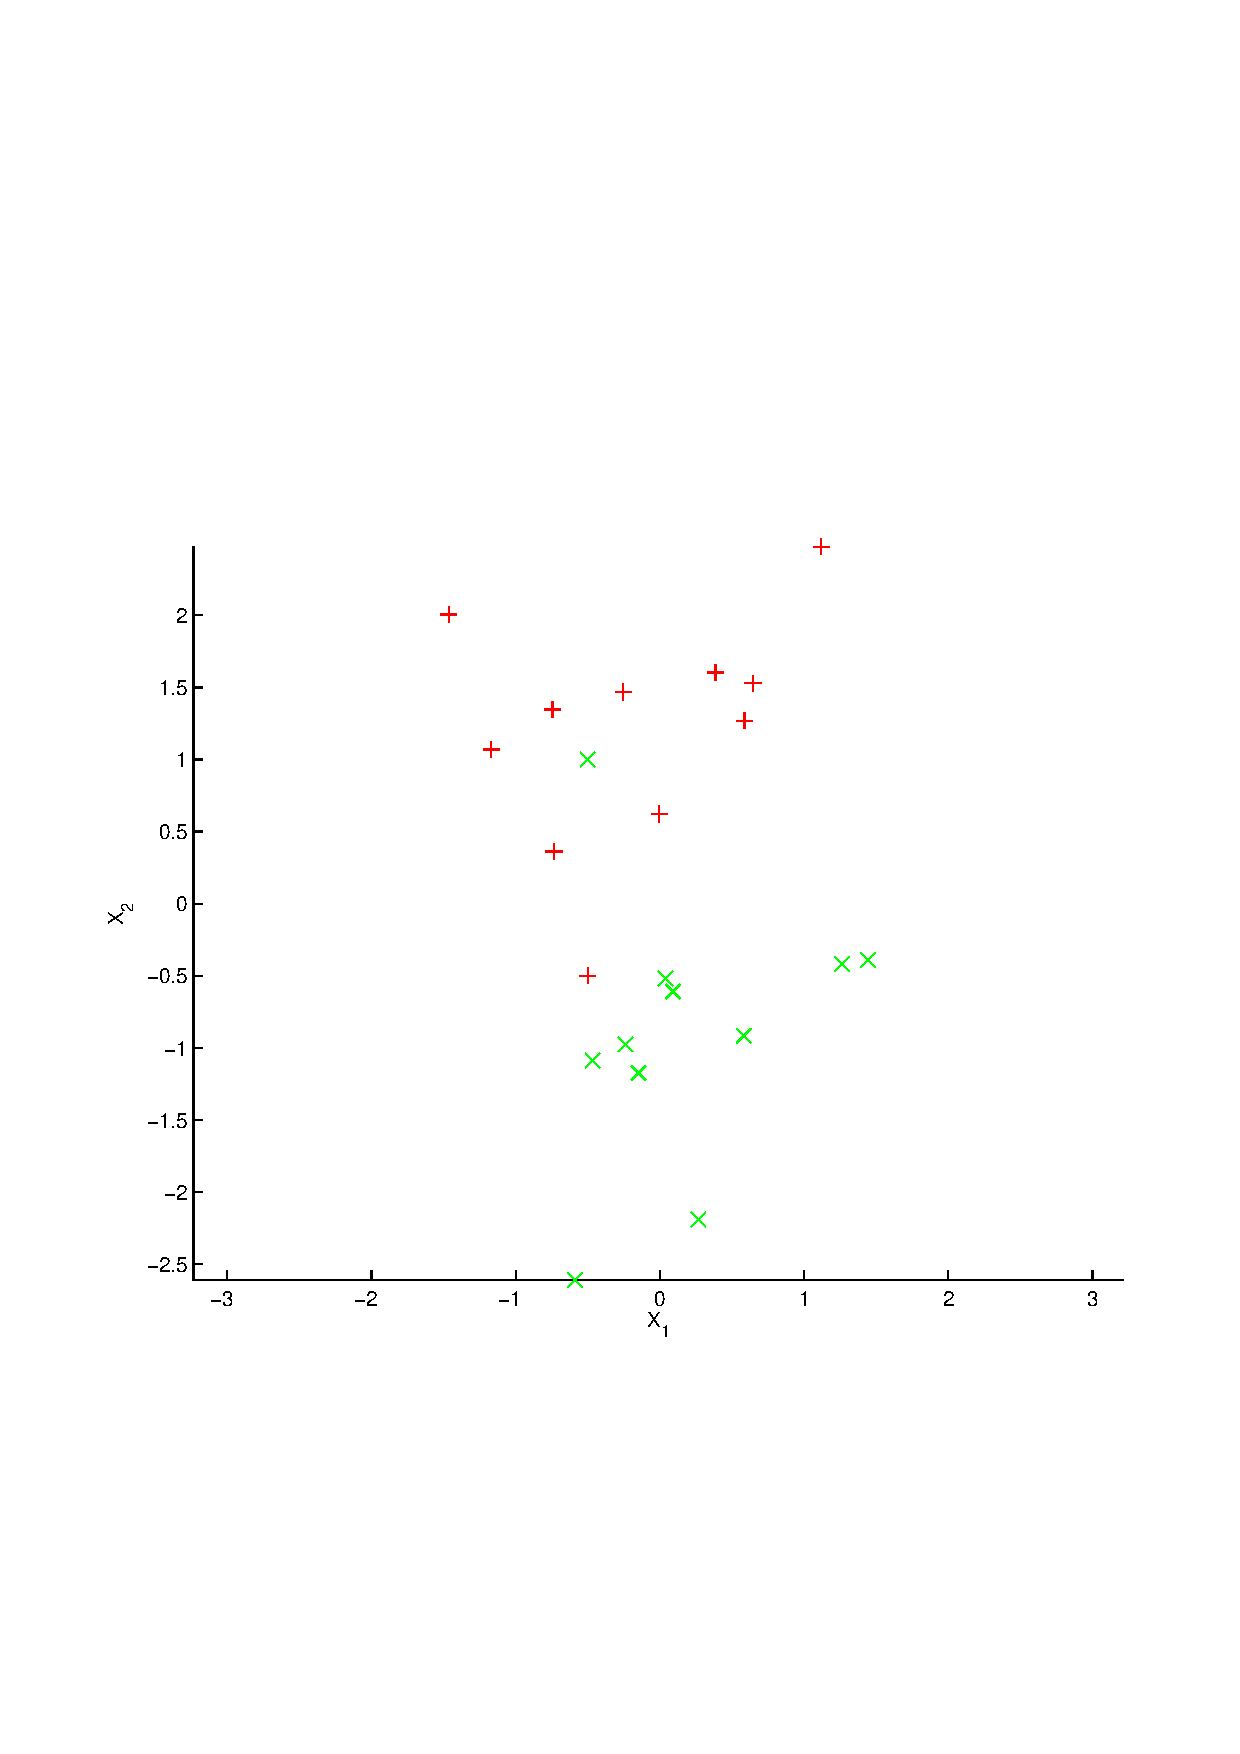
\includegraphics[width=.65\textwidth]{nonsep_svm_pb.pdf}
   \end{center}
\end{frame}


\begin{frame}
   \frametitle{Maximum margin separating hyperplane (nonseparable case)}
   \begin{block}{Solution for the nonseparable case}
   Considering a {\em soft-margin} that allows  wrong classifications
      \begin{itemize}
      \item introduction of {\em slack variables} $\xi_i\ge 0$ s.t.
     \begin{align*}
         y_i(\boldsymbol{x_i}^T \boldsymbol{\beta} + \beta_0) & \ge (1-\xi_i)
      \end{align*}
      Support vectors include now the wrong classified points, and the points inside the margins ($\xi_i > 0$)
     \item Primal problem: adding a penalty in the criterion
     $$\left\{ \begin{array}{ll}
       \min_{\bbeta,\beta_0,\xi} & \frac{1}{2} || \boldsymbol{\beta}||^2 + C \sum_{i=1}^n \xi_i,\\
       \textrm{subject to } &   y_i(\boldsymbol{x_i}^T \boldsymbol{\beta} + \beta_0)  \ge 1-\xi_i, 
      \end{array} \right.$$
      where $C>0$ is the ``cost'' parameter
      \end{itemize}
    \end{block}

\end{frame}


\begin{frame}
   \frametitle{Cost parameter (nonseparable case)}
        $$
         \textrm{Criterion to be minimized: } \quad \frac{1}{2} || \boldsymbol{\beta}||^2 + C \sum_{i=1}^n \xi_i,
      $$
   \begin{block}{Influence of the cost parameter $C>0$}
 $C$ drives the margin size, thus the number of support vectors
       \begin{itemize}
         \item $C \gg 0$~: $\sim$ underfitting (small margin, less support vectors)
         \item $C \rightarrow 0^+$~: $\sim$ overfitting (large margin, more  support vectors)
         \item $C \rightarrow +\infty$~: converges to the separable case
       \end{itemize}
       %\item $\xi_i^* = M \xi_i \leftarrow$ distance between a support vector and the margin
    \end{block}
    
    \begin{block}{Choosing the cost parameter $C>0$}
     \begin{itemize}
         \item the optimal $C$ can be estimated by cross validation
         \item[\doigt] performance might not be very sensitive to choices of $C$ (because of the rigidity of a linear boundary)
	 \item[\doigt] usually $C\approx 1$ yields a good trade-off
       \end{itemize}  
    \end{block}


\end{frame}

\begin{frame}
   \frametitle{Dual problem (nonseparable case)}
   
   Introducing the Lagrangian and substituting the first order KT conditions w.r.t. $\bbeta$, $\beta_0$, $\bxi$
   yields the dual expression
    \begin{block}{Dual optimization problem}
   $$\left\{ \begin{array}{lc}
    \max_{\balpha}    & \widetilde{L}(\balpha)  =  \sum_{i=1}^n \alpha_i  - \frac{1}{2}   \sum_{i,j=1}^n \alpha_i \alpha_j y_i y_j 
    \bx_i^T \bx_j,\\
    \textrm{subject to } & 0 \le  \alpha_i \alert{\le C} \textrm{ and } \sum_{i=1}^n \alpha_i y_i= 0. 
   \end{array}\right. $$

\begin{itemize}
 \item[\doigt] only difference w.r.t the separable case: $\alpha_i \alert{\le C}$ constraint!
 \item[\doigt]  simple convex optimization problem for which standard numerical procedure are available
\end{itemize}
 \end{block}
 
\end{frame}


\begin{frame}
   \frametitle{Optimal separating hyperplane}
    \begin{block}{Example (nonseparable case)}
    \end{block}
 \begin{minipage}{.65\textwidth}
     \begin{center}
      \includegraphics[width=\textwidth]{nonsep_svm_ann_en.pdf}
   \end{center}
 \end{minipage} \hfill
\begin{minipage}{.33\textwidth}
%\begin{center}
                 $\xi_i^* \equiv M \xi_i \leftarrow$ distance between a support vector and the margin
%                \end{center}
\end{minipage}


\end{frame}


\section{Linear discrimination: comparison of SVM vs LDA}

\begin{frame}
  \frametitle{Linear discrimination:  SVM vs LDA}
  \begin{block}{Linear discrimination}
   \begin{itemize}
    \item Linear Discriminant Analysis (LDA): Gaussian generative model
    \item SVM: criterion optimization (maximizing the margin)
   \end{itemize}
  \end{block}


\begin{minipage}{.48\textwidth}
\begin{center}
\includegraphics[width=\textwidth]{svm_margins_ann_en.pdf}\\
\textcolor{blue}{SVM}
\end{center}
\end{minipage}
\hfill
\begin{minipage}{.48\textwidth}
\begin{center}
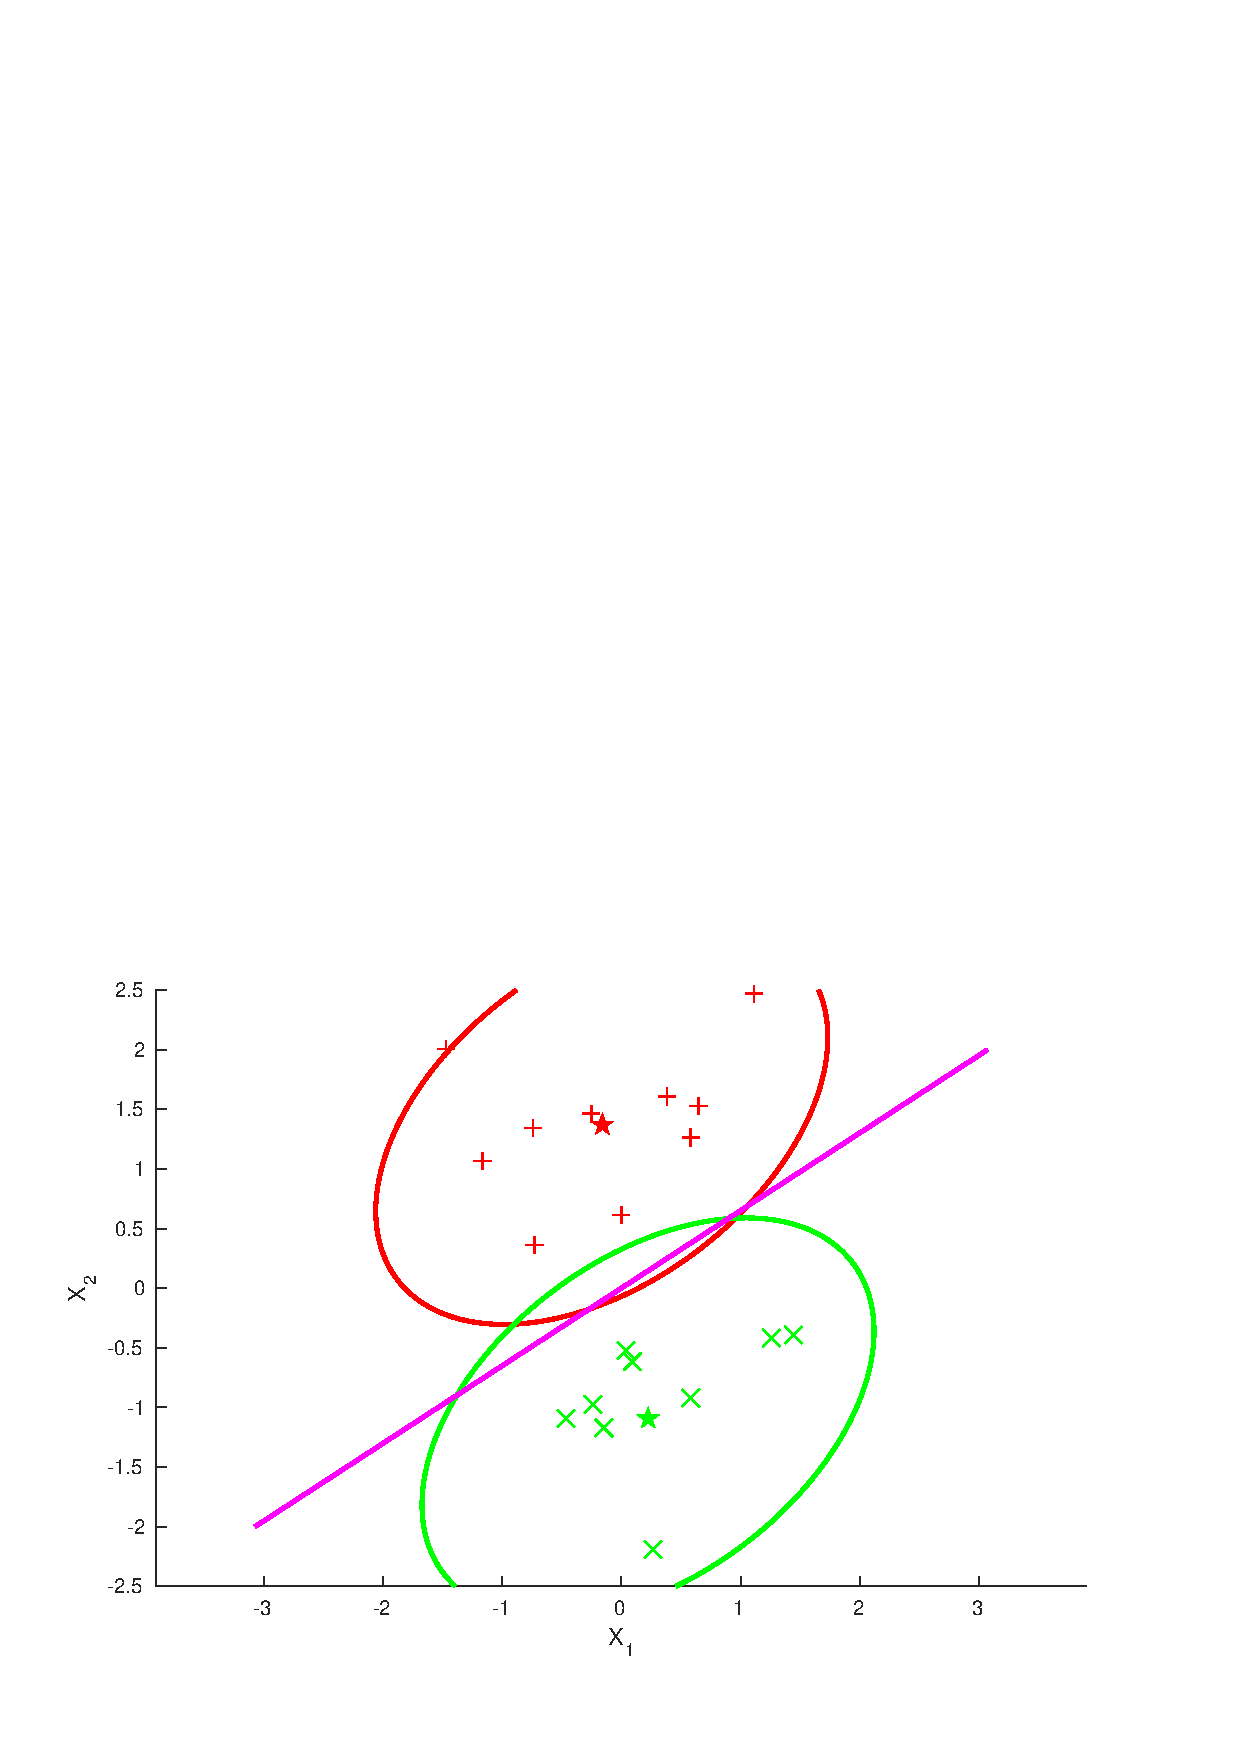
\includegraphics[width=\textwidth]{lda.pdf}\\
\textcolor{blue}{LDA}
\end{center}
\end{minipage}

\end{frame}


\begin{frame}
  \frametitle{Linear discrimination:  SVM vs LDA (Cont'd)}

\begin{block}{Adding one atypical data}
\end{block}


\begin{minipage}{.48\textwidth}
\begin{center}
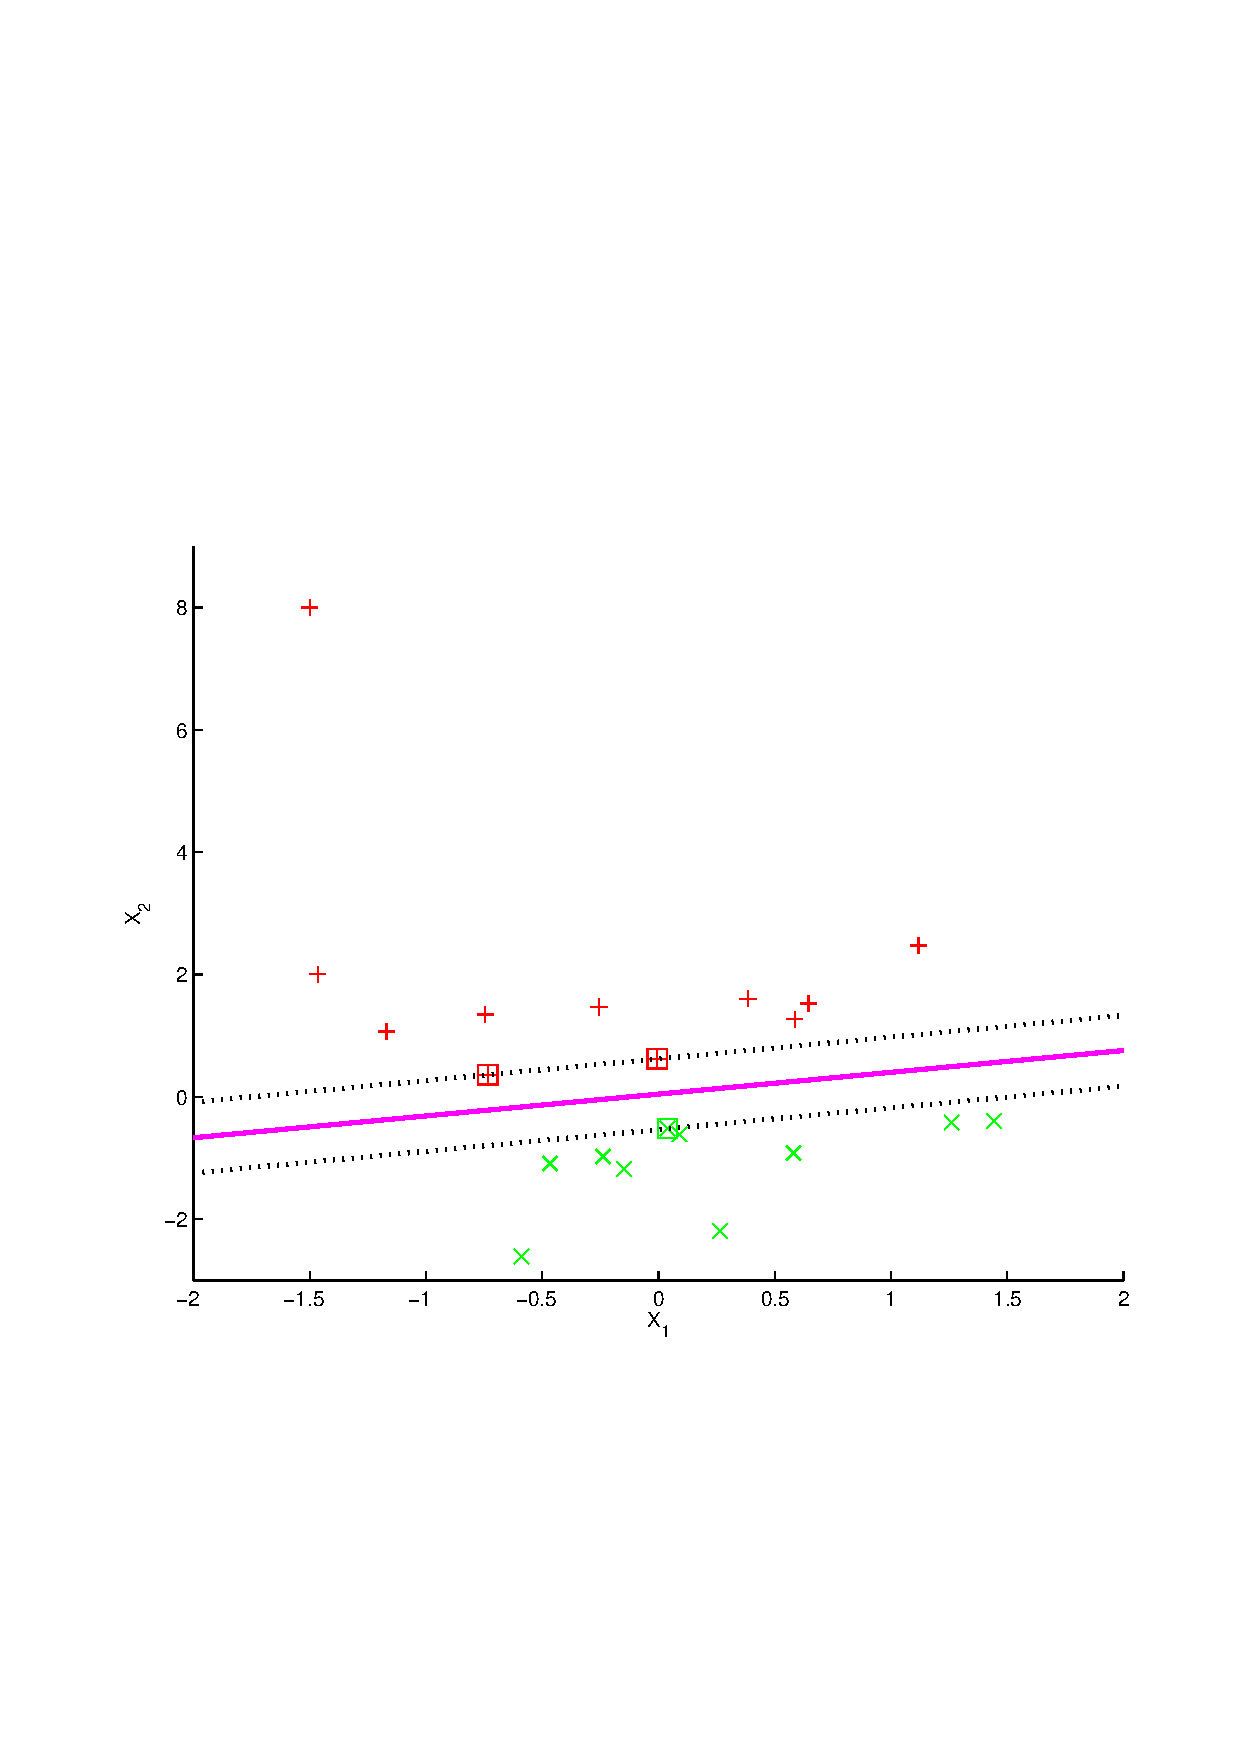
\includegraphics[width=\textwidth]{svm_margins_out.pdf}\\
\textcolor{blue}{SVM}
\end{center}
\end{minipage}
\hfill
\begin{minipage}{.48\textwidth}
\begin{center}
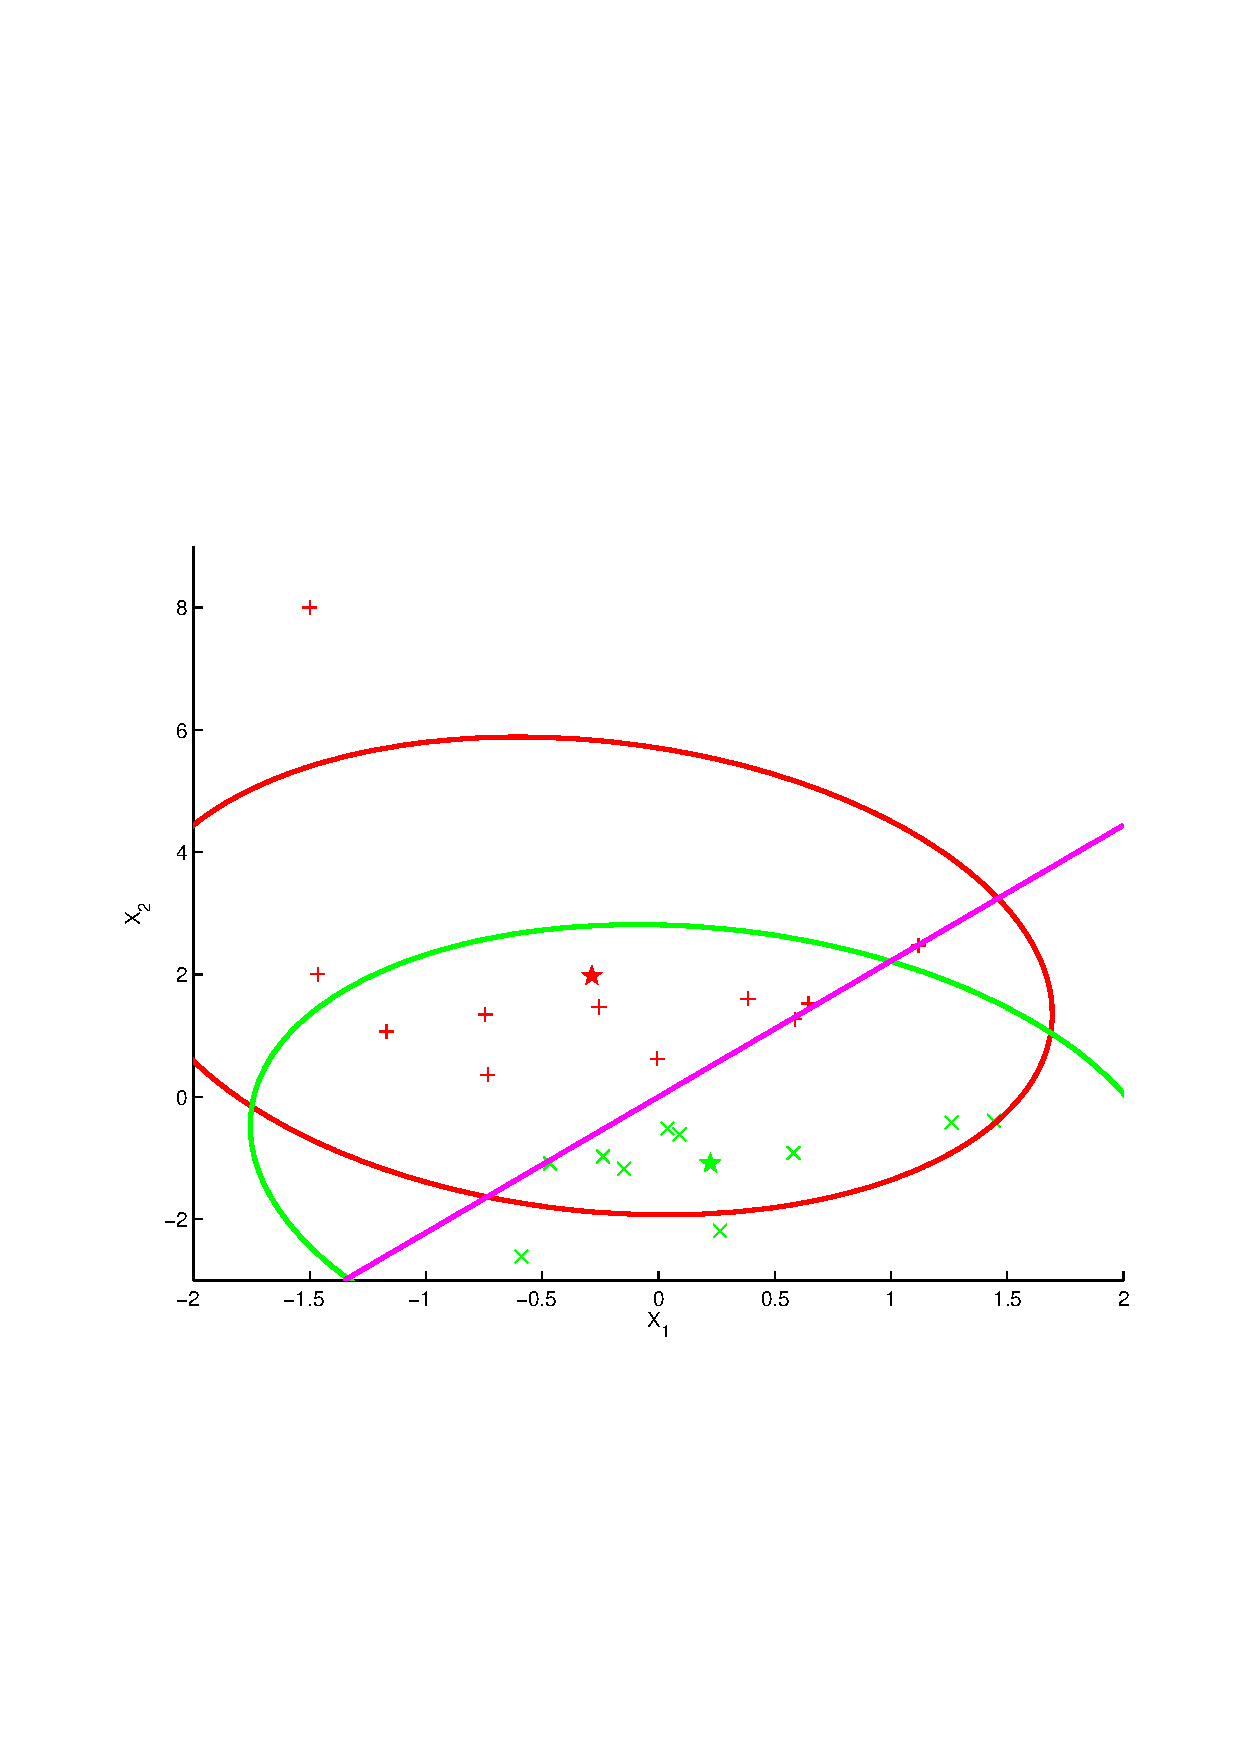
\includegraphics[width=\textwidth]{lda_out.pdf}\\
\textcolor{blue}{LDA}
\end{center}
\end{minipage}

  \begin{block}{SVM property}
   \begin{itemize}
    \item Nonsensitive to atypical points (outliers) far from the margin
    \item[\doigt] sparse method (information $\equiv$ support vectors)
   \end{itemize}
  \end{block}

\end{frame}




\section{Transformed space and Kernel function}




\begin{frame}
  \frametitle{Nonlinear discrimination in the input space}


\begin{center}
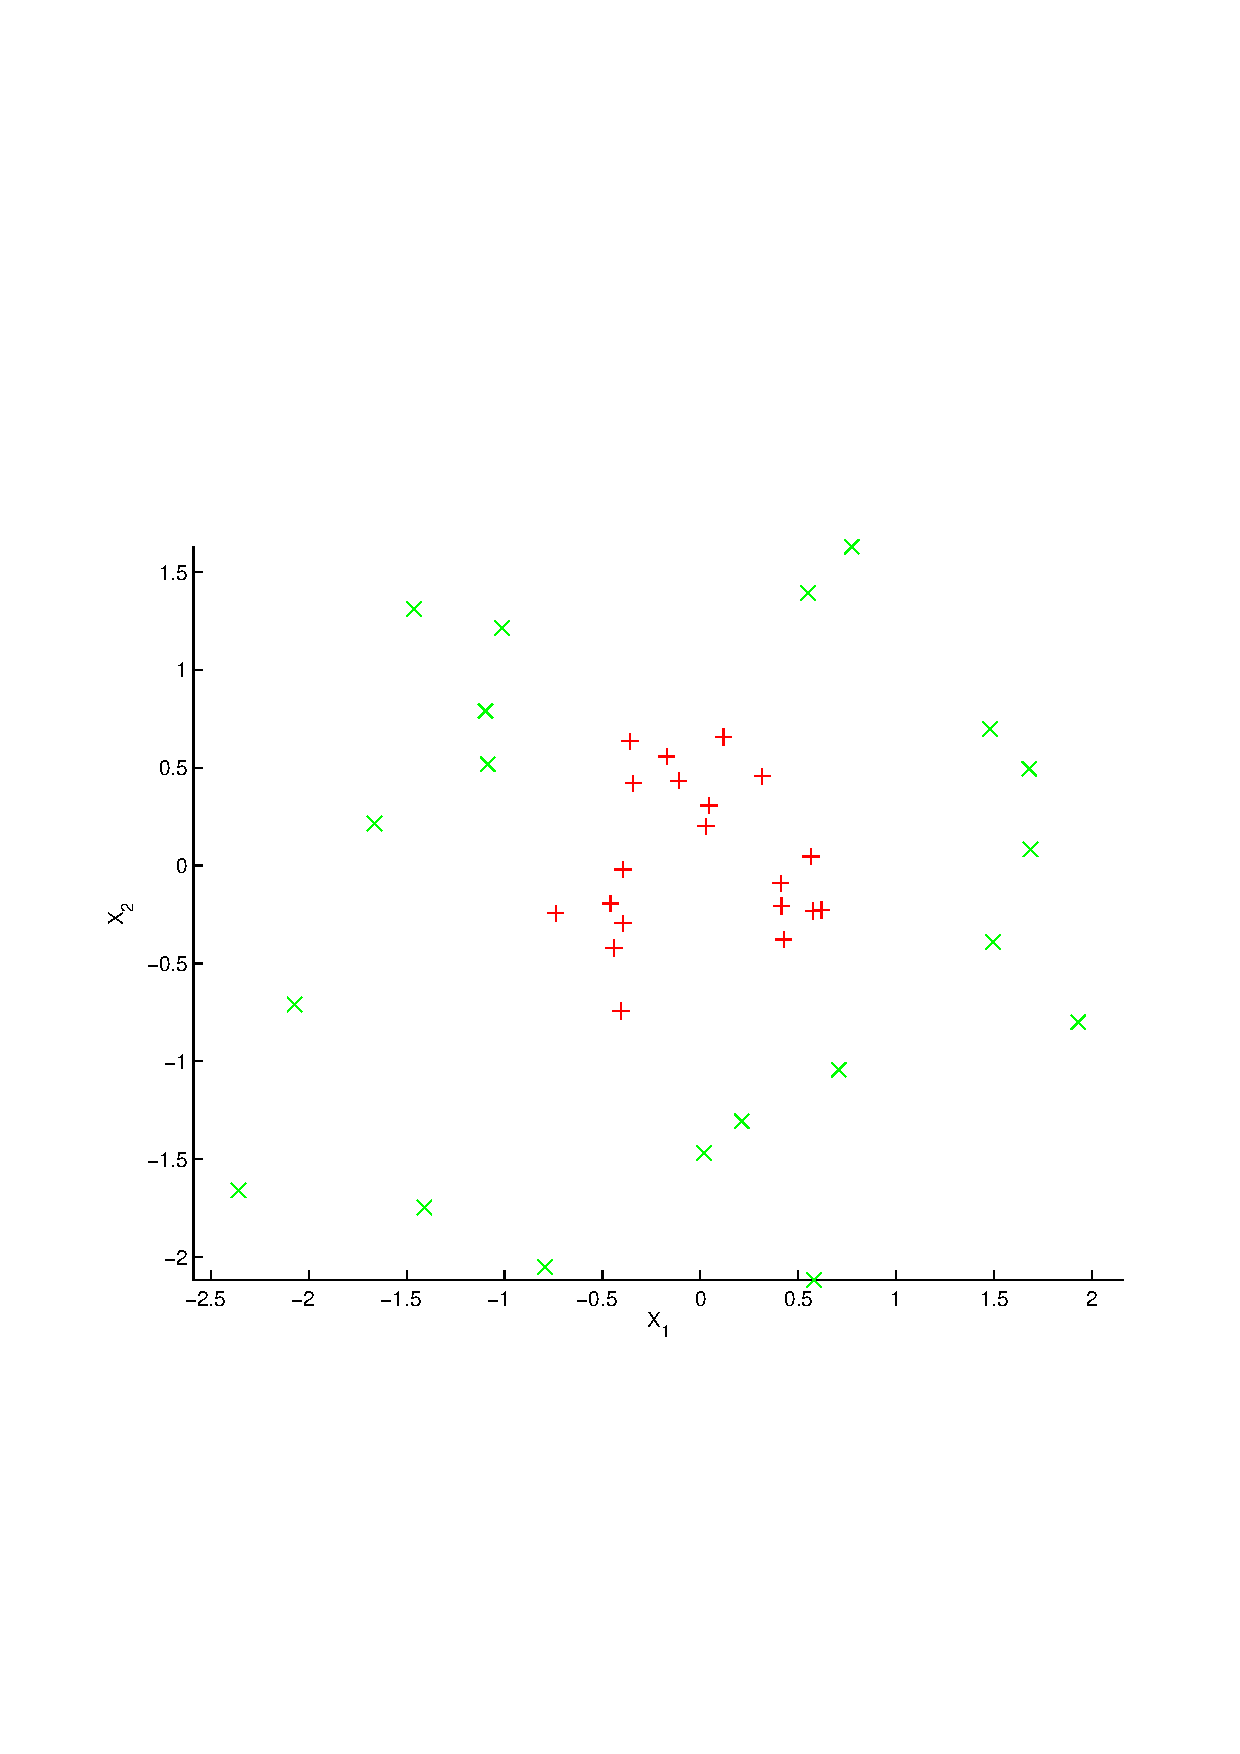
\includegraphics[width=.6\textwidth]{non_lin_pb.pdf}
\end{center}

\begin{block}{Transformed space $\mathcal{F}$}
\begin{itemize}
   \item Choice of a transformed space  $\mathcal{F}$ (feature space) where
   the linear separation assumption is more relevant
   \item Nonlinear expansion map $\phi~: \mathbb{R}^p \rightarrow \mathcal{F} $, $\bx\mapsto \phi(\bx)\leftarrow$ features
\end{itemize}


\end{block}


\end{frame}


\begin{frame}
  \frametitle{Nonlinear discrimination in the input space}

\begin{itemize}
 \item  $X \in \mathbb{R}^2$, $\phi(x)= (x_1^2,x_2^2,\sqrt{2}x_1 x_2)^T$
\end{itemize}

\begin{center}
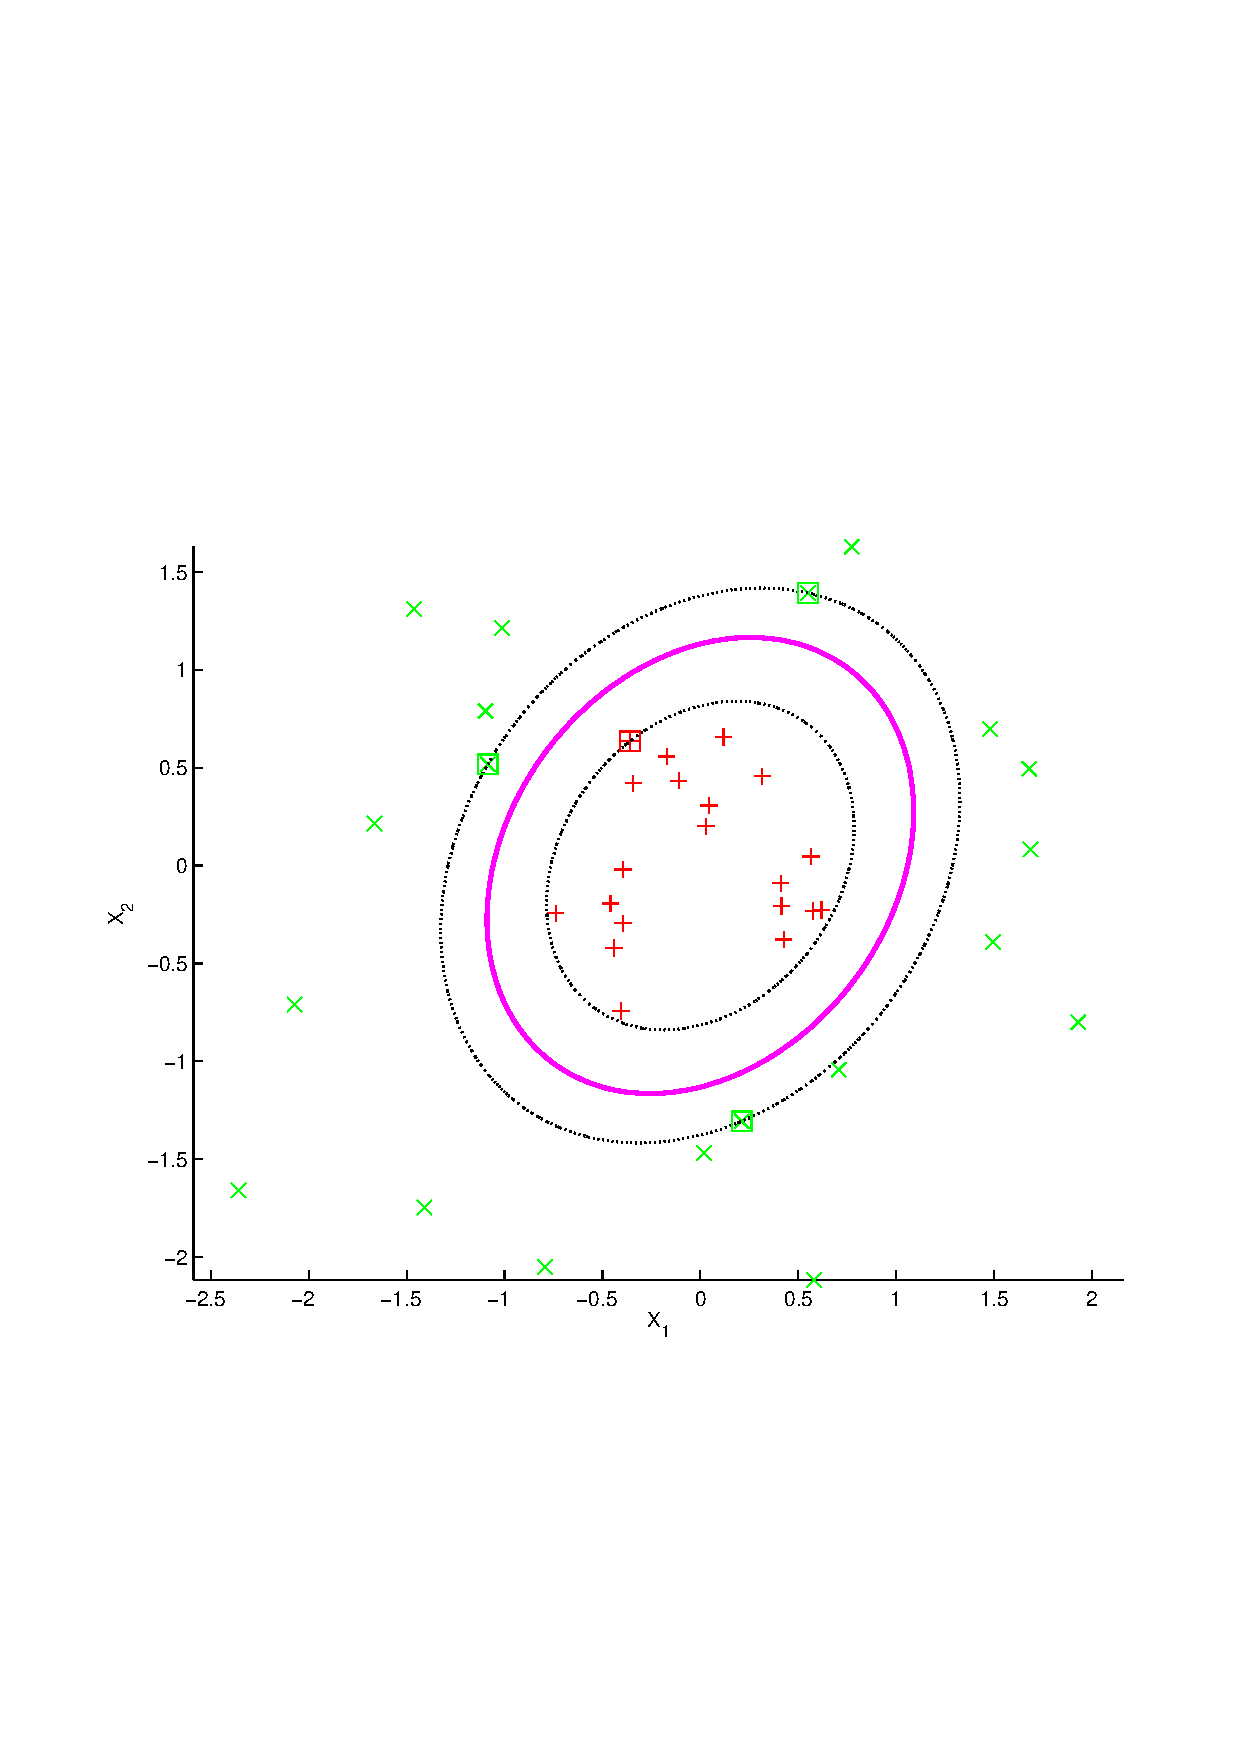
\includegraphics[width=.6\textwidth]{nonlinear_svm.pdf}\\
\color{blue}{Linear separation in the feature space $\mathcal{F}$ $\Rightarrow$
Nonlinear separation in the input space}
\end{center}


\end{frame}



\begin{frame}
  \frametitle{Kernel trick}
  
The SVM solution depends only on the \structuretext{inner product} between the input features $\phi(\bx)$ and the support vectors 
  $\phi(\bx_{\textrm{margin}})$
  
  \begin{block}{Kernel trick}
  Use of  a kernel function $k$ associated with an expansion/feature map $\phi$:
  $$\begin{array}{ccll} k:& \mathbb{R}^p \times \mathbb{R}^p  &\rightarrow& \mathbb{R}\\ 
              & (\bx,\bx') &\mapsto& \structuretext{ k (\bx,\bx') \equiv \langle \phi(\bx), \phi(\bx') \rangle}
             \end{array}$$
  and the separating hyperplane reads $h(\bx)= \sum_{i=1}^n \widehat{\alpha}_i y_i k(\bx_i,\bx)+ \widehat{\beta}_0$
  \end{block}
 
 \begin{block}{Advantages}
  \begin{itemize}
   \item computations are performed in the original input space: less  expansive than in a high 
   dimensional transformed space $\mathcal{F}$
   \item explicit representations of the feature map $\phi$ and  feature space $\mathcal{F}$ are not necessary, the only expression of $k$
   is required!
   \item[\doigt] possibility of complex transformations in possible infinite space  $\mathcal{F}$
   \item[\doigt] standard trick in machine learning not limited to SVM (kernel-PCA, gaussian process, kernel ridge regression, spectral clustering $\ldots$)
  \end{itemize}

 \end{block}


\end{frame}


\begin{frame}
  \frametitle{Choosing the Kernel function}

 \begin{block}{Mercer theorem}
 $k(\cdot,\cdot)$ should be a symmetric positive (semi-) definite function
 \end{block}

  \begin{block}{Usual kernel functions}
\begin{itemize}
 \item  Linear kernel ( $\mathcal{F} \equiv \mathbb{R}^p$)~:
 $
    k(x,x') =x^T x'
$
 \item  Polynomial kernel (dimension of $\mathcal{F}$ increases with the order $d$)
 \begin{align*}
    k(x,x') &=(x^T x')^d \quad \textrm{ or } \quad (x^T x'+1)^d
 \end{align*}
  \item Gaussian radial function ($\mathcal{F}$ with infinite dimension)
 \begin{align*}
    k(x,x') &= \exp{\left( - \gamma ||x - x'||^2\right)}
 \end{align*}
   \item  Neural net kernel ($\mathcal{F}$ with infinite dimension)
 \begin{align*}
    k(x,x') &= \tanh{\left( \kappa_1 x^T x' + \kappa_2 \right)}
 \end{align*}
\item[\doigt] optimal kernel parameters can be estimated by cross validation
\end{itemize}
 \end{block}

\end{frame}




\section*{Examples}

\begin{frame}
  \frametitle{Application: binary data  (cf course 01)}


\begin{block}{Linear kernel}
 \end{block}

\begin{center}
\includegraphics[width=.55\textwidth]{exempleBin_lin1.jpg}%\\
%\color{blue}{$C=10000$}
\end{center}

\end{frame}

\begin{frame}
  \frametitle{Application: binary data  (cf course 01)}


\begin{block}{Linear kernel}
 \end{block}

\begin{center}
\includegraphics[width=.55\textwidth]{exempleBin_lin2.jpg}%\\
%\color{blue}{$C=10000$}
\end{center}

\end{frame}

\begin{frame}
  \frametitle{Application: binary data  (cf course 01)}


\begin{block}{Polynomial kernel ($d=4$)}
 \end{block}

\begin{center}
\includegraphics[width=.55\textwidth]{exempleBin_poly4.jpg}\\
\color{blue}{$C \approx 1$}
\end{center}

\end{frame}


\begin{frame}
  \frametitle{Application: binary data  (cf course 01)}


\begin{block}{Gaussian radial kernel ($\gamma=1$)}
 \end{block}

\begin{center}
\includegraphics[width=.55\textwidth]{exempleBin_rad.jpg}\\
\color{blue}{$C \approx 1$}
\end{center}

\end{frame}

\section{Multiclass SVM}
\begin{frame}
  \frametitle{Multiclass SVM}
  \begin{itemize}
   \item $Y \in \{1,\ldots,K\}$ $\leftarrow$ $K$ classes
  \end{itemize}
   Standard approach: direct generalization by using multiple binary SVM
   \begin{block}{one-versus-all strategy}
    \begin{itemize}
    \item $K$ classifiers between one class ($+1$ label) versus all the other classes ($-1$ label)
    \item[\doigt]  classifier with the highest confidence value (e.g. the maximum distance to the separator hyperplane) assigns the class
    \end{itemize}
   \end{block}
   
   
    \begin{block}{one-versus-one strategy}
    \begin{itemize}
    \item $K(K-1)/2$ classifiers between every pair of classes
    \item[\doigt] majority vote rule: the class with the most votes determines the instance classification
    \end{itemize}
   \end{block}
  

  \end{frame}
  
  
  \section{Conclusions}
  \begin{frame}
  \frametitle{Conclusions}
  \begin{block}{SVM}
  \begin{itemize}
   \item maximum margin learning criterion $\leftarrow$ model free
   \item classification algorithm nonlinear in the original input space by performing an implicit linear classification
   in a higher dimensional space
   \item sparse solutions characterized by the support vectors
   \item popular algorithm, with a large literature 
    \end{itemize}
\end{block}

  

  \end{frame}

  
  

\end{document}
